\setcounter{num}{0}
\setcounter{numz}{0}
\begin{tcolorbox}[colframe=lightgray,colback=white,coltitle=black,title=Allgemeines:\indent Trainingsablauf Begrüßung und Ende]
	\null\vfill\null	
	\begin{tabularx}{\textwidth}{llX}
		\multicolumn{2}{l}{\textbf{Japanisch}} 	& \textbf{Deutsch}\\
		\midrule
		\ctu		& Seiza 				& Kniesitz. Füße unter dem Gesäß, Hände liegen auf den Oberschenkeln\\
		\ctu		& Mokus\={o}			& Meditation\\
		\ctu		& Mokus\={o} Yame		& Ende der Meditation\\
		\ctu a		& Sh\={o}men ni Rei		& Gruß zur Vorderseite des D\={o}j\={o}\\
		\thenum .b	& Sensei ni Rei			& Gruß zum Meister\\
		\thenum .c	& Senpai ni Rei			& Gruß zum Fortgeschrittenen (als Trainer)\\
		\ctu		& Otagai ni Rei			& Gegenseitiger Gruß\\
		\ctu		& Kiritsu				& Aufstehen\\		
		\midrule
	\end{tabularx}\\\null\vfill\null
	\begin{center}
		\parbox{\textwidth-2\tabcolsep}{Zwischen 4\,\&\,5. kann, je nach D\={o}j\={o}, ein \textit{\textquotedblleft Onegai Shimasu\textquotedblright}~zu Beginn, bzw.\,\textit{\mbox{\textquotedblleft Arigat\={o} Gozaimashita\textquotedblright}}~zum Ende des Trainings eingefügt werden - beide Begriffe sind in ihrer Übersetzung relativ unscharf, lassen sich aber ganz gut mit \textit{\textquotedblleft Ich habe eine Bitte\dots\textquotedblright}~und \textit{\textquotedblleft Danke für deine Weisheit\textquotedblright}~übersetzen. Zwischen 5.\,\&\,6. kann ein \textit{\textquotedblleft Ossu\textquotedblright}~eingefügt sein. Grundsätzlich läuft das Training in jedem D\={o}j\={o} nach diesem Schema ab und es ist wichtig, wenn man an einem Lehrgang teilnimmt, oder als Gast in einem fremden D\={o}j\={o} mittrainiert, sich an der jeweiligen Etikette zu orientieren und danach zu richten.}
	\end{center}\null\vfill\null
\end{tcolorbox}
%------------------------------------------------------------------------------
\clearpage
\pagebreak
%%------------------------------------------------------------------------------
\setcounter{num}{10}
\setcounter{numz}{0}	
\begin{tcolorbox}[colframe=lightgray,colback=white,coltitle=black,title=Allgemeines:\indent Zahlen - Angriffsstufen - Begriffe]
	\null\vfill\null	
	\begin{tabularx}{\textwidth}{lllll}		
		& \textbf{Deutsch} 	& \textbf{Japanisch} 	& \textbf{Kanji} &\multirow{13}{*}{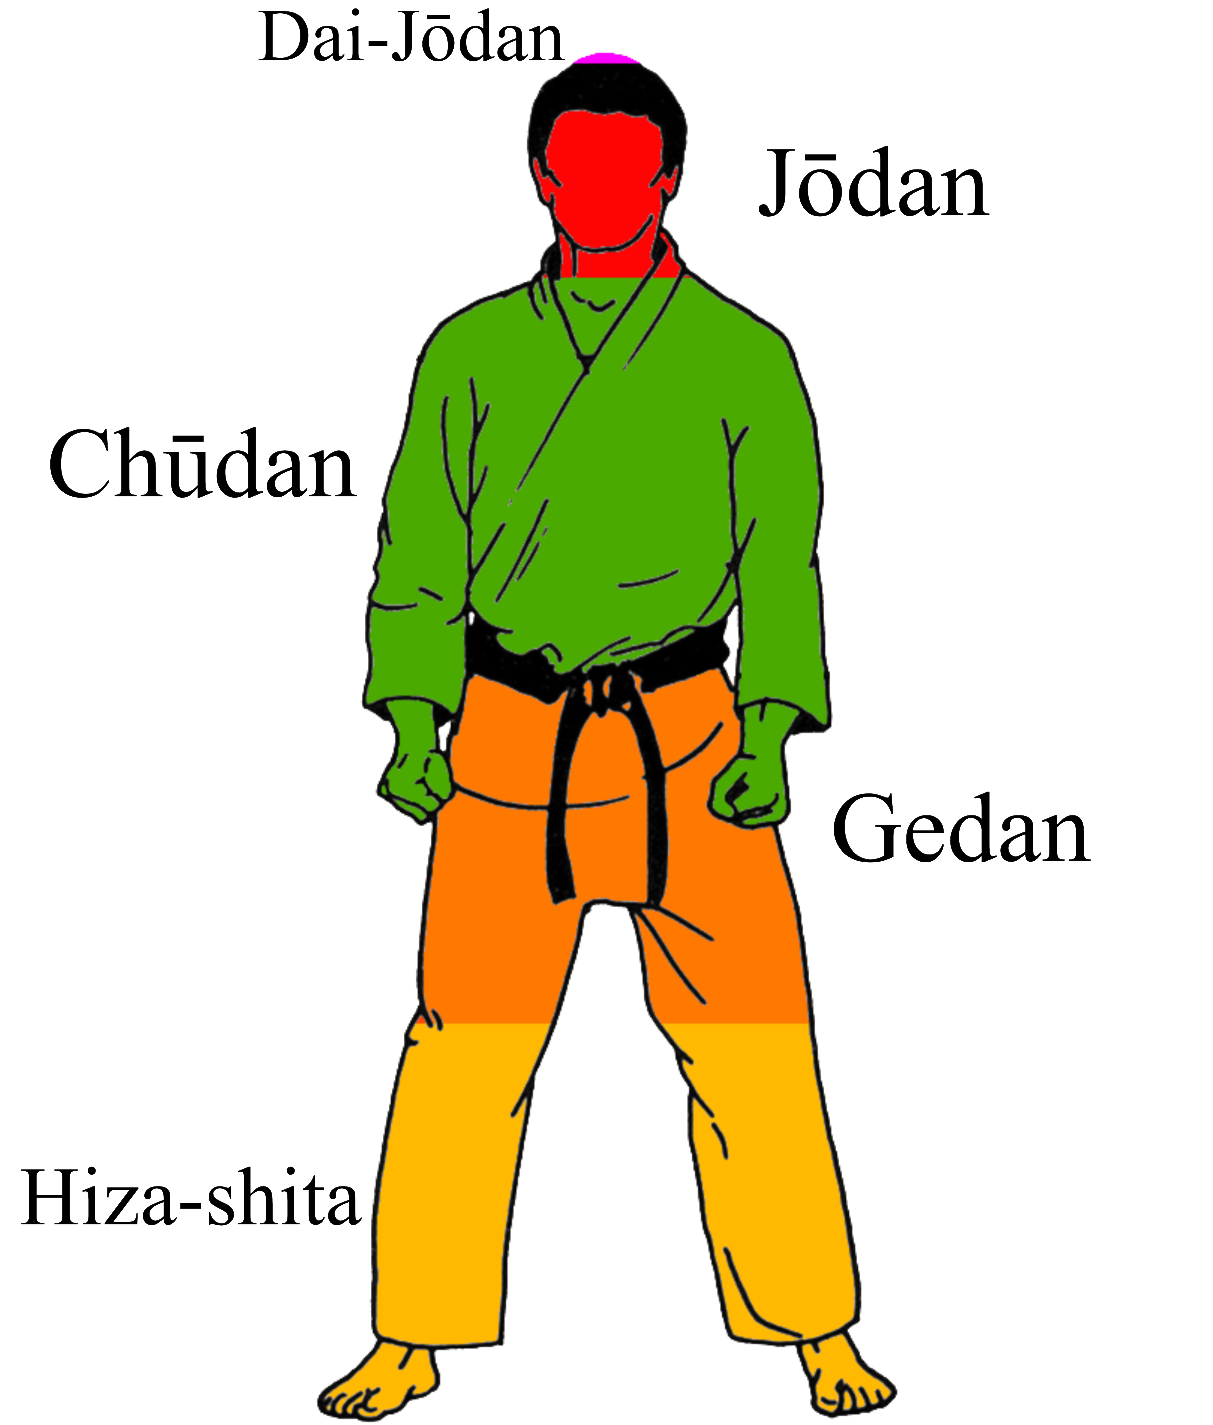
\includegraphics[height=200pt,keepaspectratio]{habersetzer_angriffsstufen_farbig}} \\
		\ctuz 	& Eins 				& Ichi 					& \begin{CJK*}{UTF8}{ipxm}\color{Navy}一\end{CJK*} 	& \\
		\ctuz 	& Zwei 				& Ni 					& \begin{CJK*}{UTF8}{ipxm}\color{Navy}二\end{CJK*} 	& \\ 
		\ctuz 	& Drei 				& San 					& \begin{CJK*}{UTF8}{ipxm}\color{Navy}三\end{CJK*} 	& \\
		\ctuz 	& Vier 				& Yon 					& \begin{CJK*}{UTF8}{ipxm}\color{Navy}四\end{CJK*} 	& \\
		\ctuz 	& Fünf 				& Go 					& \begin{CJK*}{UTF8}{ipxm}\color{Navy}五\end{CJK*} 	& \\
		\ctuz 	& Sechs 			& Roku 					& \begin{CJK*}{UTF8}{ipxm}\color{Navy}六\end{CJK*} 	& \\
		\ctuz 	& Sieben 			& Shichi 				& \begin{CJK*}{UTF8}{ipxm}\color{Navy}七\end{CJK*} 	& \\
		\ctuz 	& Acht 				& Hachi 				& \begin{CJK*}{UTF8}{ipxm}\color{Navy}八\end{CJK*} 	& \\
		\ctuz 	& Neun 				& Kyū 					& \begin{CJK*}{UTF8}{ipxm}\color{Navy}九\end{CJK*} 	& \\
		\ctuz 	& Zehn 				& Jū 					& \begin{CJK*}{UTF8}{ipxm}\color{Navy}十\end{CJK*} 	& \\
		\addlinespace
		& \multicolumn{2}{l}{G\={o}j\={u}-Ry\={u}}	& {\LARGE \begin{CJK*}{UTF8}{ipxm}\color{GKD}剛\,柔\,流\end{CJK*}}        & \\ 	
		& \multicolumn{2}{l}{Karate-D\={o}}			& {\LARGE \begin{CJK*}{UTF8}{ipxm}空\,手\,道\end{CJK*}}        & \\
		\addlinespace
		\addlinespace
		\addlinespace
		& \textbf{Deutsch} 	& \textbf{Japanisch\quad} 	& \textbf{Deutsch} 								& \textbf{Japanisch}\quad{\tiny \textcopyright\,Roland Habersetzer - Die Grundtechniken des Karate} \\
		& Rechts 			& Migi 					& Oben 												& J\={o} \\
		& Links				& Hidari 				& Mitte 											& Ch\={u} \\
		& Vorn 				& Mae 					& Unten 											& Ge [Shimo] \\
		& Hinten 			& Ushiro 				& Haken 											& Kake [Kagi, Hira] \\
		& Aufwärts 			& Age 					& Drehend / im Halbkreis 							& Mawashi\\
		& Abwärts 			& Otoshi 				& [von] Außen 										& Soto \\
		& Übungsform, fest& Kata 					& Anwendung der Kata 								& [Kata"=]Bunkai \\
	\end{tabularx}	
	\null\vfill\null
\end{tcolorbox}
%%------------------------------------------------------------------------------
\clearpage
\pagebreak
%%------------------------------------------------------------------------------
\begin{tcolorbox}[colframe=lightgray,colback=white,coltitle=black,title=Allgemeines:\indent Grundsätze und D\={o}j\={o}kun nach Miyagi Chojun]	
	\begin{footnotesize}
		\begin{tabularx}{\textwidth}{X}
			\textbf{Grundsätze des okinawanischen G\={o}j\={u}-Ry\={u}} \\
			\midrule
			Es sollte bekannt sein, dass geheime Prinzipien des G\={o}j\={u}-Ry\={u} in den Kata existieren. \\
			G\={o}j\={u}-Ry\={u} Karate-D\={o} ist eine Manifestation der harmonischen Übereinstimmung des Universums im eigenen Selbst. \\ 
			Der Weg des G\={o}j\={u}-Ry\={u} Karate-D\={o} besteht darin, den Weg der Tugend zu suchen.\\
		\end{tabularx}\null\vfill\null
		\begin{tabularx}{\textwidth}{Xr}	
			\hfill & \textbf{Geduld} \\
			\midrule
			\hfill & Du musst vor allem die Kunst der wahren und echten Geduld erlernen. \\
			\hfill & Folge dem Weg der Geduld bis zur siebten Kraft und sei nie in Eile zu lernen. \\
			\hfill & Denke immer zuerst nach und vermeide überstürztes Handeln. \\
			\hfill & Füge niemals jemandem Schaden zu oder lasse zu, dass man dir Schaden zufügt. \\
		\end{tabularx}\null\vfill\null
		\begin{tabularx}{\textwidth}{X}	
			\textbf{D\={o}j\={o}kun}\\
			\midrule
			Achte auf deine Höflichkeit mit Bescheidenheit. \\
			Trainiere dich in Anbetracht deiner körperlichen Stärke. \\
			Studiere und entwerfe ernsthaft. \\
			Sei ruhig im Geist und schnell im Handeln. \\
			Achte auf dich selbst. \\
			Lebe ein schlichtes und einfaches Leben. \\
			Sei nicht zu stolz auf dich. \\
			Übe weiter mit Geduld und Demut. \\
		\end{tabularx}\null\vfill\null
		\begin{tabularx}{\textwidth}{Xr}	
			\hfill & \textbf{Acht Gebote aus dem Bubishi}\\
			\midrule
			\hfill & Der Geist ist eins mit Himmel und Erde. \\
			\hfill & Der Kreislaufrhythmus des Körpers ist dem Zyklus von Sonne und Mond ähnlich. \\
			\hfill & Die Art des Ein- und Ausatmens ist hart und weich. \\
			\hfill & Handle im Einklang mit der Zeit und dem Wandel. \\
			\hfill & Die Techniken werden in Abwesenheit bewusster Gedanken ausgeführt. \\
			\hfill & Die Füße müssen sich vor- und zurückziehen, sich trennen und treffen. \\
			\hfill & Den Augen entgeht nicht einmal die kleinste Veränderung. \\
			\hfill & Die Ohren hören gut in alle Richtungen. \\
		\end{tabularx}
	\end{footnotesize}
\end{tcolorbox}
%%------------------------------------------------------------------------------
\clearpage
\pagebreak
%%------------------------------------------------------------------------------
\setcounter{num}{0}
\setcounter{numz}{0}	
\begin{tcolorbox}[colframe=lightgray,colback=white,coltitle=black,title=Allgemeines:\indent weitere Begriffe aus dem Japanischen]
	\begin{tabularx}{\linewidth}{lXlX}%{p{0.20\linewidth}p{0.20\linewidth}Xp{0.20\linewidth}p{0.20\linewidth}}
		Japanisch	& Deutsch	& Japanisch&Deutsch\\
		\midrule
		Awase-Uke&	unterstützende Abwehr	&	Enbusen	&	Schrittdiagramm der Kata\\
		Gaiwan	& Außenseite des Unterarms	&	Go-No-Sen	&	Initiative \textbf{nach} dem Angriff\\
		Hajime!&	Anfangen!	&	Happo-Kumite	& Kampf in alle Richtungen\\
		Junbi-Und\={o}	& Aufwärmen	&	Kakie	& schiebende Hände\\
		Kime	&	Impuls zur Technik setzen	& Kiritsu & Steht auf!\\
		Mawatte	& Wendung&	Mond\={o}& Lehrgespräch\\
		Morote	& beidhändig	& Muchimi & klebende Hände\\
		Renzoku Geiko	& Flowübungen zum Automatisieren & Sen-No-Sen & Initiative \textbf{vor} dem Angriff\\
		Shizentai	& natürliche Körperhaltung&Sun-Dome & Technik abstoppen  kurz vor dem Ziel\\
		Yakusoku Kumite & abgesprochenes Kämpfen & Yame	& Stop!\\
%		\hrulefill&\hrulefill&\hrulefill&\hrulefill&\hrulefill\\
	\end{tabularx}
%\rule{\linewidth}{6pt}\\
%\rule{\textwidth}{6pt}
\end{tcolorbox}
%%------------------------------------------------------------------------------
%\begin{tcolorbox}colframe=lightgray,colback=white,coltitle=black,title=Allgemeines:\indent D\={o}j\={o}kun nach Funakoshi Gichin \textmd{{\footnotesize \textit{auch Sh\={o}t\={o}  Nij\={u} Kun}}}]
%	\null\vfill\null	
%	\begin{tabularx}{\textwidth}{X}
%		Karate beginnt und endet mit Respekt. \\
%		Im Karate gibt es keinen ersten Angriff. \\ 
%		Karate ist ein Helfer der Gerechtigkeit. \\
%		Erkenne zuerst dich selbst, dann den anderen. \\
%		Die Kunst des Geistes kommt vor der Kunst der Technik. \\
%		Es geht einzig darum, den Geist zu befreien. \\
%		Unglück geschieht immer durch Unachtsamkeit. \\
%		Denke nicht, dass Karate nur im D\={o}j\={o} stattfindet. \\
%		Karate üben heißt, es ein Leben lang zu tun. \\
%		Verbinde dein alltägliches Leben mit Karate, dann wirst du geistige
%		Reife erlangen. \\
%		Karate ist wie heißes Wasser, das abkühlt, wenn du es nicht ständig
%		warmhälst. \\
%		Denke nicht darüber nach zu gewinnen, sondern denke darüber nach, wie
%		man nicht verliert. \\
%		Wandle dich abhängig vom Gegner. \\
%		Der Kampf hängt von der Handhabung des Treffens und des Nicht-Treffens
%		ab. \\
%		Stelle dir deine Hand und deinen Fuß als Schwerter vor. \\
%		Sobald man vor die Tür tritt, findet man ein Vielzahl von Feinden vor. \\
%		Feste Stellungen gibt es für Anfänger, später bewegt man sich natürlich. \\
%		Die Kata darf nicht verändert werden, im Kampf, jedoch gilt das Gegenteil. \\
%		Hart \& weich, Spannung \&  Entspannung, langsam \& schnell, alles in
%		Verbindung mit der richtigen Atmung. \\
%		Denke immer nach und versuche dich ständig an Neuem. \\
%	\end{tabularx}\\\null\vfill\null
%\end{tcolorbox}
%%------------------------------------------------------------------------------
%\clearpage
%\pagebreak
%%------------------------------------------------------------------------------
